Programming for SIEMENS Tecnomatix Process Simulate was initially desirable, as it exposes a Microsoft .NET Framework compatible API. 
This allows developers to choose any of the many .NET languages to create Process Simulate plugins, including but not limited to C\#, C++, F\#, Visual Basic, Iron Python. 
All the code in this work is written in C\#.

\section{Writing Plug-ins}
Any .NET assembly can be a Process Simulate plugin, as it only looks at the contents. 
A class library project is ideal for this as there is no benefit for any other project type. 
For Process Simulate to pick up the assembly, it should be located in \emph{DotNetCommands} or \emph{DotNetExternalApplications} directories and registered with the application. 
These directories and any following paths are relative to the programs installation directory. 
Typically this would be \cls{C:/Program Files/Tecnomatix 13.0/eMPower}, but might differ based on the user's choice at install-time.

To register an external application or a command with Process Simulate, we need to use a utility \emph{CommandReg.exe} which comes with the application. 
When you launch the program a dialog, similar to the one presented in Figure~\ref{fig:CommandReg}, will appear. 
In this dialog we select the compiled file, we want to load, pick the commands located in the assembly and choose a filename for the configuration XML file which will be newly created. 
This XML allows the settings to be moved between computers easily. \\

\begin{figure}[H]
    \caption{CommandReg Utility}
    \centering
    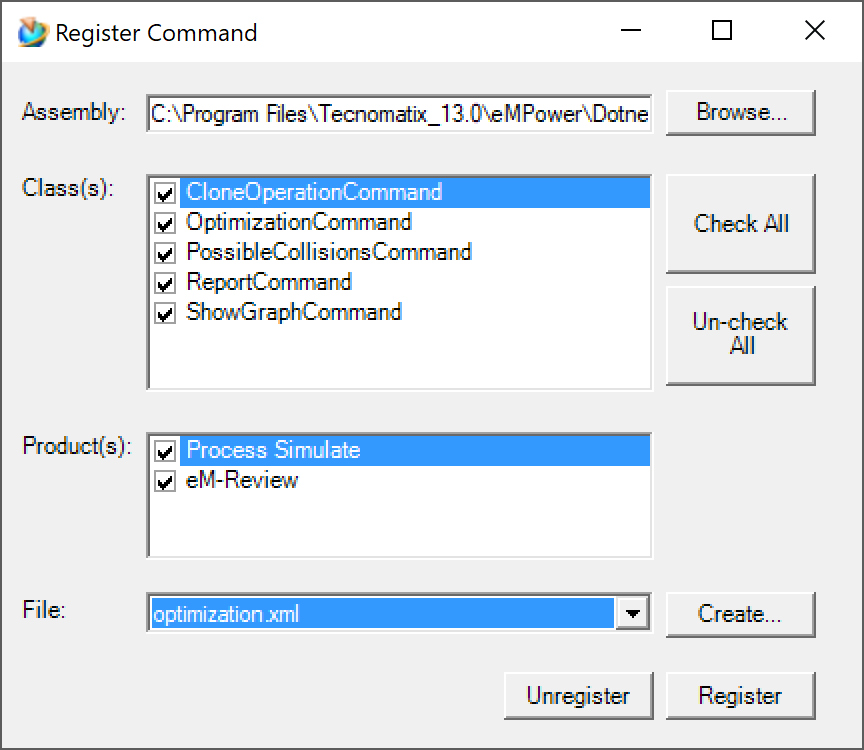
\includegraphics{commandreg}
    \label{fig:CommandReg}
\end{figure}

After we registered our commands, we need to configure our workspace to be able to use them. 
More specifically, we need to choose where the application should display buttons for the commands in the ribbon menu. 
This can be achieved by right-clicking the ribbon to invoke the context menu and selecting the \emph{Customize Ribbon} option as shown in Figure~\ref{fig:CustomizeRibbonContextMenu}.
A dialog like you see in Figure~\ref{fig:CustomizeRibbonDialog} will appear where the user can add new commands to the ribbon and customize the layout. 
The newly registered actions will appear in the list. Unfortunately, there is no grouping available. 
Therefore the best option is to look for the exact names in the alphabetically sorted list. \\

\begin{figure}[H]
    \caption{Customize the Ribbon}
    \centering
    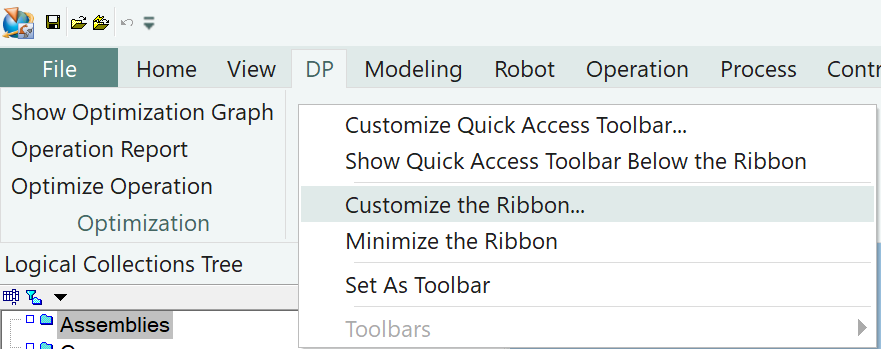
\includegraphics{customizeribbon}
    \label{fig:CustomizeRibbonContextMenu}
\end{figure}

\begin{figure}[H]
    \caption{Add commands to the Ribbon}
    \centering
    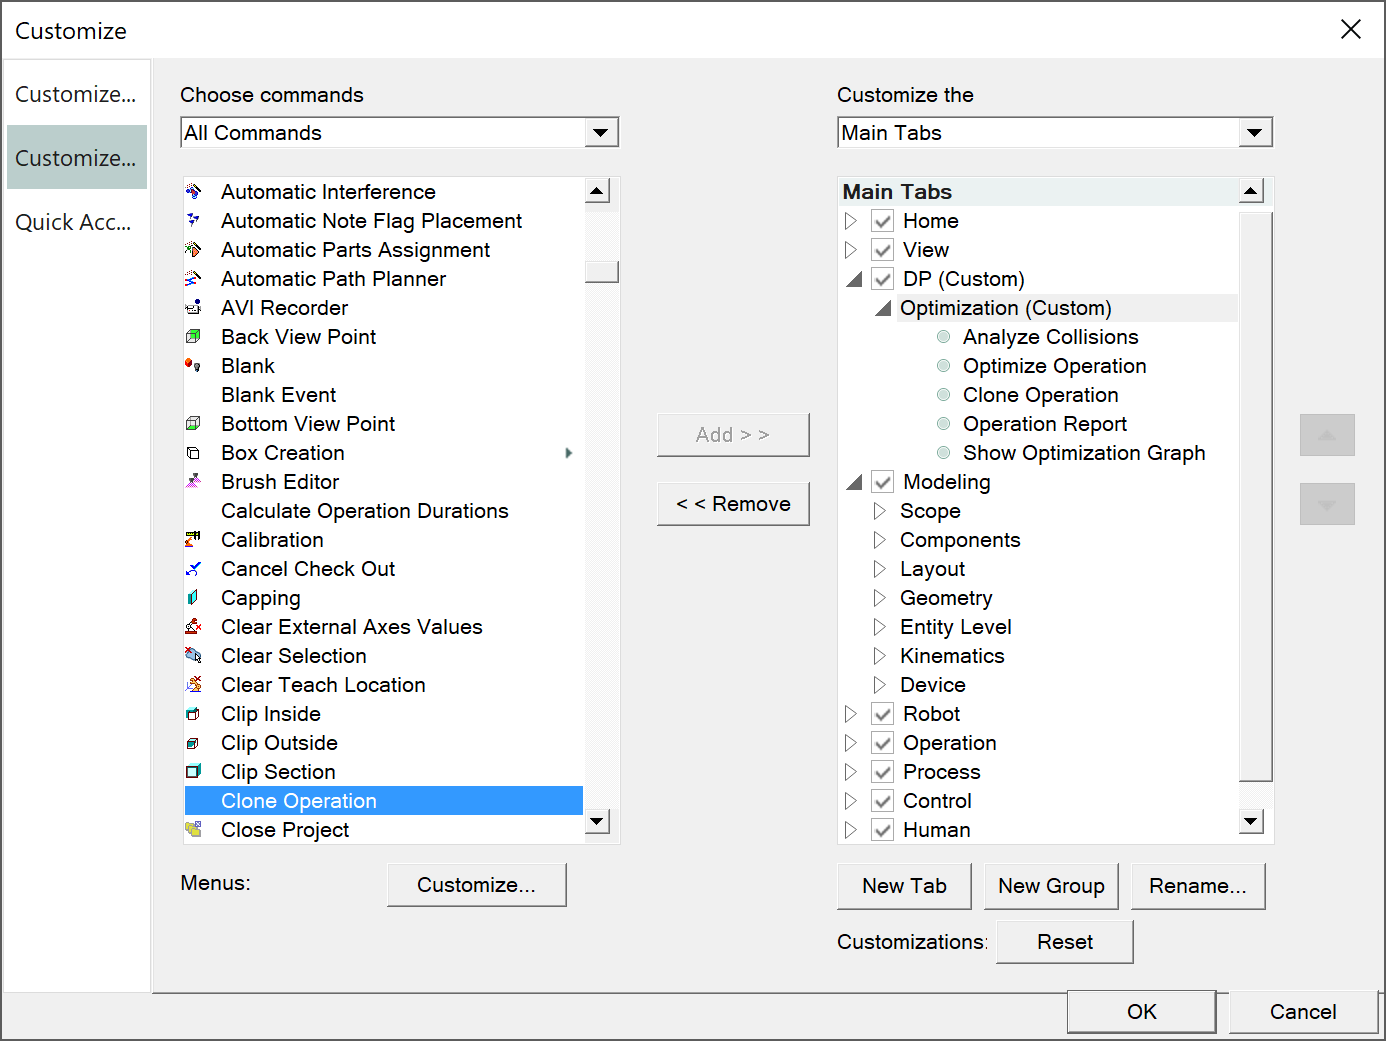
\includegraphics[width=\textwidth]{addcommands}
    \label{fig:CustomizeRibbonDialog}
\end{figure}

Next, we will look like at how to code new commands so that Process Simulate would recognize them. 
For this, we first need to include a reference for the main dynamically linked library \cls{Tecnomatix.Engineering.dll}. 
Writing plugins for the application revolves mostly around this one library, as it contains all the classes used to interact with the application. 
There are multiple types of commands which are recognized by Process Simulate.
They are named based on the UI elements they represent and range from buttons to combo boxes. 
Most commonly used command type is the button, which Figure~\ref{fig:CodeCommand} shows implemented.
To create a button command we have to create a new class and inherit the \cls{TxButtonCommand} abstract class.
After the user clicks the button, the \cls{Execute} method will be invoked, where we put our business logic. \\

\begin{figure}[H]
    \caption{Example Command}
    \centering
    \begin{minted}[breaklines]{csharp}
public class MyCommand : TxButtonCommand
{
    public override String Category { get; } = "My Category";
    public override String Name { get; } = "My Command";
    public override void Execute(Object cmdParams)
    {
    }
}
    \end{minted}
    \label{fig:CodeCommand}
\end{figure}

\section{API}

This section is dedicated to acquainting the reader with the most important classes in the \cls{Tecnomatix.Engineering.dll} library. It is not the only library available for the plugin developers, but apart from edge-cases it's the only one developers need. It allows developers to extract information from the application instance that loaded the plugin and currently the opened project. It includes routines to control some of the functions of the application.

\subsection{TxApplication}
\cls{TxApplication} is a static class which serves as the main entry point to the application. This class can be readily described as the root of a tree. It holds instances of sub-services in its static properties bound to the current application instance. It also contains routines which control application specific behavior. In Figure~\ref{fig:CodeTxApplication} I picked out the most important properties and presented their signature, as I believe that for a person with development experience this is the most valuable information, and the easiest to imagine.

\begin{figure}[H]
    \caption{TxApplication API}
    \centering
    \begin{minted}[breaklines]{csharp}
public sealed class TxApplication
{
    public static TxDocument ActiveDocument { get; }
    public static TxSelection ActiveSelection { get; }
    public static TxApplicationEvents ApplicationEvents { get; }
    public static TxOptions Options { get; }
    public static string StatusBarMessage { set; }
    public static void RefreshDisplay()
}
    \end{minted}
    \label{fig:CodeTxApplication}
\end{figure}

\begin{itemize}

\item \cls{ActiveDocument} is the pivotal property of this object.
It contains information about the currently opened study and allows the plugin to manipulate it. The features of this object are described in Chapter~\ref{ch:TxDocument}, which talks about the \cls{TxDocument} type.

\item \cls{ActiveSelection} allows the plugin to see what the user selected or modify the selection. This feature is especially useful when used as part of the plugins user interface, allowing the user to pick inputs for the plugin by selecting them in the application.

\item \cls{ApplicationEvents} property provides binding actions to important application events. Chapter~\ref{ch:TxApplicationEvents} goes into more detail about how to use this property.

\item \cls{Options} contains a hierarchy of objects used to retrieve and set application options. These mimic the options found in the \cls{Settings} dialog of the application. Chapter~\ref{ch:TxOptions} goes into more detail.

\item \cls{StatusBarMessage} is a simple String. Modifying this property will make the text appear in the status bar area of the application. It is a simple, but effective, way to communicate with the user unobtrusively.

\item \cls{RefreshDisplay()} causes all panels in the application to redraw using the latest data.

\end{itemize}

\subsection{TxSelection}

The \cls{TxSelection} class controls the current selection. All different kinds of items can be selected simultaneously. For this reason, the API includes this specialized class allowing the developers to interact with all kinds of selections fairly easily. In Figure~\ref{fig:CodeTxSelection} I prepared a filtered definition of the class.

\begin{figure}[H]
    \caption{TxSelection API}
    \centering
    \begin{minted}[breaklines]{csharp}
public sealed class TxSelection{
    public void Clear();
    public void AddItems(TxObjectList items);
    public void SetItems()
    public void RemoveItems()
    public ITxObject GetLastPickedItem();
    public TxTransformation GetLastPickedLocation();
    public TxObjectList GetPlanningItems();
    public TxObjectList GetAllItems();
    public TxObjectList GetOrderedItems();
    public event TxSelection_ItemsSetEventHandler ItemsSet;
    public event TxSelection_ItemsAddedEventHandler ItemsAdded;
    public event TxSelection_ItemsRemovedEventHandler ItemsRemoved;
}
    \end{minted}
    \label{fig:CodeTxSelection}
\end{figure}

\begin{itemize}

\item \cls{GetOrderedItems()} gets the objects that are currently selected.
In addition to that, this routine returns only the loaded objects, in their engineering representation in the order they were selected.

\item \cls{GetAllItems()} returns the same information, but does not guarantee order.

\item \cls{GetPlanningItem()} returns planning representations like 
\cls{TxPlanningPart} or \cls{TxPlanningResource}, in contrast to the aforementioned routines which return engineering representations like \cls{TxRobot} or \cls{TxComponent}.

\item \cls{GetLastPickedLocation()} returns coordinates of the last picked object.

\end{itemize}

\subsection{TxApplicationEvents}
\label{ch:TxApplicationEvents}

The \cls{TxApplicationEvents} class wraps multiple application events. The events include the closing of the application which the plugin can use to clean up temporary resources. The application exit request can also be intercepted should the user have some unsaved work in the plugin. You can see the class definition in Figure~ref{fig:CodeTxApplicationEvents}. Additionally, Figure~\ref{fig:CodeTxApplicationEventsUsage} shows how the events in this class are used.

\begin{figure}[H]
    \caption{TxApplicationEvents API}
    \centering
    \begin{minted}[breaklines]{csharp}
public sealed class TxApplicationEvents
{
    public event TxApplication_ExitingEventHandler Exiting;
    public event TxApplication_ExitRequestEventHandler ExitRequest;
    public event TxApplication_ExitingEventHandler Closing;
}
    \end{minted}
    \label{fig:CodeTxApplicationEvents}
\end{figure}

\begin{itemize}

\item \cls{Exiting} Occurs when the application is about to exit.

\item \cls{ExitRequest} Occurs before the application is about to exit.
To reject the request to exit, specify \cls{false} for the \cls{Approve} field of the event arguments.

\item \cls{Closing} Occurs when a project is closed.

\end{itemize}

\begin{figure}[H]
    \caption{TxApplicationEvents Usage}
    \centering
    \begin{minted}[breaklines]{csharp}
class Demo()
{
    public Demo()
    {
        TxApplication.ApplicationEvents.Exiting += (sender, e) => {
            Save();
        };
        TxApplication.ApplicationEvents.ExitRequest += (sender, e) => {
            e.Approve = !unsavedWork;
        };
    }
}
    \end{minted}
    \label{fig:CodeTxApplicationEventsUsage}
\end{figure}

\subsection{TxOptions}
\label{ch:TxOptions}

The \cls{TxOptions} provides access to the application options as they mirror the options in the \cls{Options} dialog.
These options include collision checking configuration, units used, simulation and so on.
Please note that spot welding options aren't available in RobotExpert, only in Process Simulate. Figure~\ref{fig:CodeStopOnCollision} shows the usage of and points out the option I found the most useful. It ensures the simulation player stops playing when it reaches the first collision.

\begin{figure}[H]
    \caption{TxOptions Usage}
    \centering
    \begin{minted}[breaklines]{csharp}
TxApplication.Options.Collision.StopOnCollision = true;
    \end{minted}
    \label{fig:CodeStopOnCollision}
\end{figure}

\subsection{TxDocument}
\label{ch:TxDocument}

The \cls{TxDocument} class represents a study. 
When talking about the \cls{TxApplication.ActiveDocument} object this would be the currently open study. 
Under the document, we can find all physical
objects, operations, manufacturing features, and robotic programs. 
It also facilitates access to objects that have a single instance per document.

\begin{figure}[H]
    \caption{TxDocument API}
    \centering
    \begin{minted}{csharp}
public sealed class TxDocument
{
    public ITxOperation CurrentOperation { get; }
    public TxOperationRoot OperationRoot { get; }
    public TxPhysicalRoot PhysicalRoot { get; }
    public TxMfgRoot MfgRoot { get; }
    public TxCollisionRoot CollisionRoot { get; }
    public TxSimulationPlayer SimulationPlayer { get; }
}
    \end{minted}
    \label{fig:CodeTxDocument}
\end{figure}

\begin{itemize}

\item \cls{OperationRoot} is the root of the operation tree

\item \cls{PhysicalRoot} is the root of the physical object tree

\item \cls{MfgRoot} is the root of the manufacturing features tree.

\item \cls{ColisionRoot} is the root of the collision pairs.
It is used to determine where the workspace currently contains a collision.

\item \cls{SimulationPlayer} is used to simulate operations and events.
At any given moment there is a single, current simulation player, with which all commands and viewers work.
\end{itemize}

\subsection{Operations}

Operations in Process Simulate inherit the \cls{ITxOperation} interface. When they have children, as all operations except on the point level do, they also implement the \cls{ITxObjectCollection} interface which serves as a nongeneric \cls{List} specific to the Process Simulate .NET API. All operations have a name and a description.

\subsubsection{TxOperationRoot}

This class is the root of all operations.
Its children are usually of type \cls{TxCompoundOperation}.
We can query all children with the \cls{GetAllDescendants()} or \cls{GetDirectDescendants()} methods.
Operations can't be created using the new keyword invoking a constructor.
To create a new operation use the \cls{CreateXOperation()} on a class that implements \cls{ITxOperationCreation}, like for example \cls{TxOperationRoot}. The X in \cls{CreateXOperation()} is the specific operation type you are trying to create, and the classes contains methods for all operation types. For example, if we wanted to create a \cls{GenericRoboticOperation} we would use the  \cls{CreateGenericRoboticOperation} method.
The created operation still needs to be inserted into a specific place in the operation tree.

\begin{figure}[H]
    \caption{TxOperationRoot API}
    \centering
    \begin{minted}[breaklines]{csharp}
bool CanCreateXOperation()
TxXOperation CreateXOperation(XCreationData creationData)
GetDirectDescendants(ITxTypeFilter filter)
GetAllDescendants(ITxTypeFilter filter)
//usage:
TxCompoundOperation newOperation =TxApplication.ActiveDocument.OperationRoot.CreateCompoundOperation(newTxCompoundOperationCreationData("name"));
foreach (ITxOperation op inTxApplication.ActiveDocument.OperationRoot.GetDirectDescendants(newTxNoTypeFilter()))
{
}
    \end{minted}
    \label{fig:CodeTxOperationRoot}
\end{figure}


\subsubsection{TxCompoundOperation}

This operation groups a set of operations (its children) into a logical group. They can also specify dependencies and offsets within the parent.

\subsubsection{TxContinuousRoboticOperation}

This path operation contains an ordered list of points.
It has a robot assigned which will carry out the whole sequence of the points.
In the object model, it contains a set of child links, each having a reference to a source and target operations.
These links are read only but can be read and manipulated using the \cls{GetChildAt()} and \cls{MoveChildAfter()} functions.
Timing offsets and durations are read-only which are captured after a simulation. Changing operation speeds won't recalculate this value, a new simulation needs to be performed. 

\subsubsection{TxRoboticViaLocationOperation}

This operation is used to avoid obstacles since a normal operation goes for a direct approach to the target point which can result in collisions.
It simply navigates the robots head to a designated point.

\subsubsection{TxObjectFlowOperation}

This operation is used for moving products from one location to another.
The operation specifies how the object is supposed to be gripped with \cls{GripFrame} (=\cls{TxFrame}) and \cls{GripFrameType} (=\cls{GeometricCenter}) properties.
The product will be moved through points specified by objects of type \cls{TxObjectFlowLocationOperation} that are children of the operation (as \cls{IEnumerable}).
